\section{Tickets}
\label{sec:tickets}

In the HOPR protocol, nodes that have staked funds within a payment channel can issue tickets that are used for payment to other nodes. Tickets are used for \lcnameref{sec:incentives:probabilistic}; every ticket is bound to a specific payment channel and cannot be spent elsewhere. Tickets are redeemable at most once and lose their value when the associated payment channel is closed or when the commitment is reset. A commitment is a secret on-chain value used to verify whether a ticket is a winner or not when an attempt is made to redeem it.

\begin{figure}[H]
      \centering
      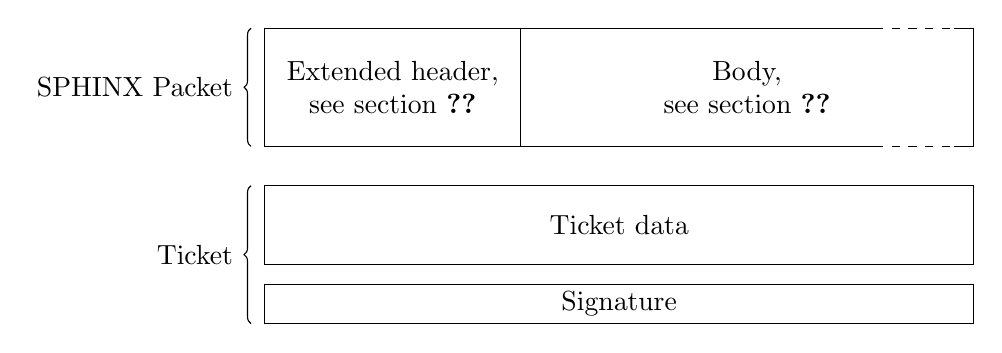
\begin{tikzpicture}[every text node part/.style={align=center}]
            \def\width{9}
            \def\headerWidth{9}
            \def\headerHeight{1.5}
            \def\headerOffset{3.25}
            \def\dashOffset{4.5}
            \def\dashWidth{1}

            \def\ticketDataHeight{1}
            \def\ticketSignatureHeight{0.5}

            \draw[decoration={brace,raise=5pt,mirror},decorate] (0,0) -- node[left=8pt] {SPHINX Packet} (0,-\headerHeight);

            \draw (0,0) rectangle (\headerOffset,-\headerHeight) node [midway] {Extended header,\\see section \ref{sec:incentives:proofofrelay}};
            \path [shape=rectangle] (\headerOffset,0) rectangle (\headerWidth,-\headerHeight) node [midway] {Body,\\see section \ref{sec:sphinx:payload}};

            \draw (\headerOffset+\dashOffset,-\headerHeight) -- (\headerOffset,-\headerHeight) -- (\headerOffset,0) -- (\headerOffset+\dashOffset,0);

            \draw [dashed] (\headerOffset+\dashOffset,0) -- (\headerOffset+\dashOffset+\dashWidth,0);
            \draw [dashed] (\headerOffset+\dashOffset,-\headerHeight) -- (\headerOffset+\dashOffset+\dashWidth,-\headerHeight);

            \draw (\headerOffset+\dashOffset+\dashWidth,-\headerHeight) -- (\headerWidth,-\headerHeight) -- (\headerWidth,0) -- (\headerOffset+\dashOffset+\dashWidth,0);

            \begin{scope}[shift={(0,-\headerHeight-0.5)}]
                  \def\padding{0.25}

                  \draw[decoration={brace,raise=5pt,mirror},decorate] (0,0) -- node[left=8pt] {Ticket} (0,-\ticketDataHeight-\padding-\ticketSignatureHeight);

                  \draw (0,0) rectangle (\headerWidth,-\ticketDataHeight) node [midway] {Ticket data};

                  \draw (0,-\ticketDataHeight-\padding) rectangle (\headerWidth,-\ticketDataHeight-\ticketSignatureHeight-\padding) node [midway] {Signature};
            \end{scope}
      \end{tikzpicture}
      \caption{Schematic overview of a mixnet packet that is sent together with a ticket.}
\end{figure}

\subsection{Ticket Issuance}
\label{sec:tickets:issuance}

Before a node is able to issue tickets for another node, it needs to lock funds to cover for the current as well as future tickets in the smart contract. Locking funds is considered equal to staking tokens in the HOPR network as it allows the node to send packets and act as relayer. By locking tokens in the smart contract, the node creates a unidirectional payment channel towards the recipient and is thus able to convince the recipient that it is eligable to issue tickets.

As ticket issuance happens without any interaction with the blockchain, it is the duty of the node who receives the ticket to check whether there were any tokens locked on-chain and to keep track about previously issued tickets. If there is no record on-chain about any locked funds or if the sum of the received tickets exceed the amount of tokens that were locked on-chain, the node should refuse the ticket.

Tickets are sent together with a mixnet packet and include the incentive for processing and forwarding the packet to the next downstream node. Hence, to meet the \lcnameref{sec:intro:securitygoals}, neither issuance nor redemption must be linkable to the creation or processing of mixnet packets. Therefore, each ticket is given a winning probability, which means that not every received ticket leads to a claimable incentive and, moreover, those tickets who turn out to be a loss cover the missed incentives of other tickets. This mechanism is not only beneficial in terms of privacy but also helps to keep transaction costs due to on-chain interactions minimal.

When issuing a ticket, the issuer determines the intended value $value$ of ticket and sets:

$$ ticketData.value := \frac{value(ticket)}{winProb} $$

where $winProb$ refers to the chosen winning probability and $ticketData.value$ is the value that is embedded in the ticket.

The ticket issuer creates a data structure $ticketData$ and creates the ticket as $ticket = (ticketData,\mathsf{Sig}_{Issuer}(ticketData))$. The following explains the data structure $ticketData$.

\begin{figure}[H]
      \centering
      \begin{tabular}{|l|c|c|}
            \hline
            \textbf{Value}                                    & \textbf{Ethereum datatype} & \textbf{size (in bytes)} \\
            \hline
            \hline
            \nameref{sec:tickets:issuance:recipient}          & address                    & 20 bytes                 \\
            \nameref{sec:tickets:issuance:challenge}          & bytes32                    & 32 bytes                 \\
            \nameref{sec:tickets:issuance:ticketepoch}        & uint256                    & 32 bytes                 \\
            \nameref{sec:tickets:issuance:ticketvalue}        & uint256                    & 32 bytes                 \\
            \nameref{sec:tickets:issuance:winningprobability} & uint256                    & 32 bytes                 \\
            \nameref{sec:tickets:issuance:ticketindex}        & uint256                    & 32 bytes                 \\
            \nameref{sec:tickets:issuance:channelepoch}       & uint256                    & 32 bytes                 \\
            \hline
            \hline
            Signature $r$                                     & bytes32                    & 32 bytes                 \\
            Signature $s$                                     & bytes32                    & 32 bytes                 \\
            Recovery value $v$                                & uint8                      & 1 byte                   \\
            \hline
      \end{tabular}
      \caption{Structure of $ticketData$.}
\end{figure}

\paragraph{Recipient}
\label{sec:tickets:issuance:recipient}

The Ethereum address of the recipient which can be derived from the recipient's public key. This makes sure that the ticket is valid for exactly one payment channel, the one from issuer to recipient. Note that Ethereum addresses are computed as

$$ addr = keccak256( uncompressedPublicKey).slice(12,32)$$

(the last 20 bytes of the keccak256 hash of the uncompressed ECDSA public key).

\paragraph{Challenge}
\label{sec:tickets:issuance:challenge}

Tickets are issued locked: the included incentive is not yet claimable but their validity can be verified. The ticket states a challenge which needs to be solved by the party who redeems the ticket. This mechanism servers as a building block for Proof of Relay as described in section \ref{sec:incentives:proofofrelay}.

\paragraph{Ticket epoch}
\label{sec:tickets:issuance:ticketepoch}

Ticket redemptions relies on providing the opening to an on-chain commitment by the party who redeems the ticket. To make sure that the party who wants to redeem tickets, is always able to compute the opening to a commitment, it is possible to renew the stored on-chain commitment.

As this allows the redeemer to change the entropy that is used to determine whether a ticket is a win or not, the ticket issuer signs the current ticket epoch stored in the smart contract, with the effect that tickets lose its value once the stored commitment gets renewed.

\paragraph{Ticket value}
\label{sec:tickets:issuance:ticketvalue}

The ticket value is given by the intended $value$ divided by the winning probability $winProb$ in the base unit of the token, which is $10^{-8}$. Hence, sending $10$ HOPR means sending $10 * 10^8$ HOPR.

\paragraph{Winning probablity}
\label{sec:tickets:issuance:winningprobability}

The proportion of tickets which lead to an actual payout is determined by their winning probability. Their value is given as the inverse of the winning probability, e.g. $10$ instead of $0.1 = 1/10$.

\paragraph{Ticket index}
\label{sec:tickets:issuance:ticketindex}

Each ticket is labeled by an ongoing serial number, the \textit{ticket index}. The ticket index is set by the ticket issuer and stored in the smart contract once the ticket gets redeemed. It is the duty of the ticket recipient that the index is increased with every ticket. If this is not the case, the ticket recipient should refuse the ticket since redeeming a ticket with an index $i$ invalidates all tickets with index $i' \le i$.

\paragraph{Channel epoch}
\label{sec:tickets:issuance:channelepoch}

Payment channels can get opened and closed as often as their participants like to. See section \ref{sec:incentives:channels} for more information. To make sure that tickets from previous channel incarnations lose their once the channel is reopened, the ticket includes the current channel epoch counter and the smart contract considers the ticket invalid if the signed channel epoch does not match the stored channel epoch.
\subsection{Ticket Validation}
\label{sec:tickets:validation}

Tickets are used to convince its recipient that it will receive the promised incentive, once the challenge is solved. As ticket issuance happens without any on-chain interaction, it is the duty of the recipient to decide whether it accepts the ticket or resuses it.

Ticket validation runs through two states: receiving the ticket without knowing the response to the given challenge stated as $ticket.challenge$, \lcnameref{sec:tickets:validation:locked}, and once the response is known, \lcnameref{sec:tickets:validation:unlocked}.

\paragraph{Validation of Locked Tickets}
\label{sec:tickets:validation:locked}

Due to the lack of a response to the stated challenge, the node is neither able to decide whether the ticket is going to be a win nor claim it on-chain to receive the incentives. Nevertheless, the node can use the embedded information to validate the ticket economically. Therefore, the node at first extracts the winning probability as

$$ticket.winProb = \frac{ticket.invWinProb}{2^{256} - 1} $$

which leads $ value(ticket) = ticket.value \cdot ticket.invWinProb $. If the node considers $value(ticket)$ inappropriate, i.e. because it does match the expected amount, or if winning probability is set too high or too low, it should refuse the ticket.

As ticket issuance happens without any on-chain interaction and thus, there is no guarantee that there is any payment channel at all and that this payment channel has enough tokens Locked. Therefore, the recipient needs to check that before considering a ticket valid. In addition, there might be previous tickets, denoted as $stored$, that are not yet redeemed. Hence, the recipient needs to check that

$$ channel.amount \le value(ticket) + \sum_{t \ \in \ stored} value(t)$$

In addtion, as tickets are issued using an ongoing serial number, the recipient must check that $ticket_i.index > \max(ticket_{i-1}.index,0)$ and refuse the ticket otherwise.

It remains to show that the ticket issuer indeed knows any $response$ that solves $ticket.challenge$. This is especially relevant if the ticket issuer was given the challenge by a third party, i.e. the creator of a mixnet packet. For this section, this specific topic is out scope and covered in section on \lcnameref{sec:incentives:proofofrelay}.

\paragraph{Validation of Unlocked Tickets}
\label{sec:tickets:validation:unlocked}

Once the $response$ to $ticket.challenge$ is known, i.e. after receiving a packet acknowledgement, the node is able determine whether the ticket is going to be a winner. To check this, the node first computes the next $opening$ to the current value $commitment$ stored in the smart contract and checks that

$$ \mathsf{keccak256} ( \ \mathsf{keccak256}(ticketData) \ || \ solution \ || \ opening \ ) < ticket.winProb $$

If true, the node can consider the ticket to be a winner and store it for later use. In case the ticket turned out to be a loss, there is no added value to it and the node can safely drop it. Note that losing tickets are a integral part of the mechanism and do not reduce the average payout to the ticket recipient. This is the case because $value(tikcet)$ is given by the expected value and hence the asymptotic payout does not change.
\subsection{Ticket Redemption}
\label{sec:tickets:redemption}

After running through the validations of the previous section, the node $n$ ends up with a set of stored tickets which it considers to be a win, hence

$$ stored := \{ t \in Tickets \ | \ isWinner(t) \land t.recipient = n \}$$

Each ticket $t$ is given a  \lcnameref{sec:tickets:issuance:ticketindex}, which means tickets need to be redeemed in order which is why the node first creates an ordered set $ordered$ out of the set $tickets$ and proceeds with the first ticket.

Redemption means that the node now proves for each $t \in stored$ one-by-one to the smart contract that $t$ is indeed a win. If successful, the smart contract transfers the stated incentives to the account of the node, see paragraph \lcnameref{sec:tickets:redemption:assettransfer}.

In contrast to ticket recipients, the smart contract considers a ticket only valid if the redeemer is able to provide a $response$ that solves $ticket.challenge$ and a value $opening$ that opens the most recent $commitment$ stored on-chain. Note that the smart contract thereby acts as a trusted third party that forces the node reveal additional cryptographic material despite the signature of the ticket is valid. This is possible because the blockchain consensus makes it infeasible to add state changes which have not been the result of a method execution in the smart contract.

\paragraph{Challenge}
\label{sec:tickets:redemption:challenge}

Solving a challenge $C$ means finding a value $r \in \mathbb{F}$ such that $r \cdot G =C$. Hence, in order to check this equation, the smart contract needs to compute a scalar multiplication of an elliptic curve point, which is as of writing of the paper not directly available within Ethereum.

Instead, Ethereun allows to efficiently implement a function $mul'$:

$$ mul': x \in \mathbb{F} \mapsto ethAddr (x \cdot G)$$

where $ethAddr: \{0,1\}^{64} \mapsto \{0,1\}^{20}$ maps uncompressed elliptic curve points to Ethereum addresses. Hence, the smart contract compares the computed Ethereum address against the challenge stated in the ticket.

\paragraph{Issuer signature}
\label{sec:tickets:redemption:signature}

By computing $C' = mul'(response)$ the smart contract is able to recompute the hash of the ticket as

\begin{multline*}
      ticketHash = keccak256 (recipient \ || \ C' \ || \ ticketEpoch \ || \ amount \ || \\
      invWinProb \ || \ index \ || \ channelEpoch)
\end{multline*}

and is thus able by using the provided signature to recover the public key of the ticket issuer. By now having both Ethereum addresses, the one of the issuer and the one of the recipient, the smart contract is able to compute the identifier $channelId$ of the utilized payment channel.

\paragraph{Payment channel validation}
\label{sec:tickets:redemption:channel}

As the previous steps were computed without any feedback to the computed values, the computed $channelId$ will either lead to a non-existing entry in case there is no such channel known to the blockchain, or to a record of a payment channel. Due to the usage of a collision-resistant hash function, it is assumed to be infeasible for an attacker to find a second pre-image that maps the ticket hash to a specific $channelId$. Hence, either the challenge is correct and there is a payment channel or any of the previous conditions is not met.

If $channelId$ leads to a payment channel record, the smart contract checks that $channel.state = OPEN$  and $channel.amount \le ticket.amount$ and rejects the ticket otherwise.

\paragraph{Replay protections}
\label{sec:tickets:redemption:replay}

A ticket can be valid due to valid signature and correct $response$, but as it controls an asset transfer and thereby initiates on-chain state changes, it must be valid exactly \textit{once}.

Each ticket is given an ongoing serial number $i$ and each ticket redemption sets the on-chain value $channel.index$ to $ticket.index$ if $ticket.index > channel.index$. Otherwise, the ticket is rejected.

Analogously, each reincarnation of the payment channel, i.e. a sequence of $open$ and $close$, increases the channel epoch counter. To turn tickets issued for previous incarnations of the payment channel invalid, the smart contract rejects all tickets with $ticket.channelEpoch \neq channel.epoch$

Last but not least, each renewal of the on-chain commitment increases the ticket epoch counter. To prevent from the ticket issuers from ticket recipients resetting the ticket epoch counter to values that they find more beneficial, e.g. in order to tweak the ticket's winning probability and turn previously losing tickets into winning ones, the smart contract rejects all tickets for which $ticket.ticketEpoch \neq channel.ticketEpoch$.

\paragraph{Commitment}

By opening a payment channel from ticket issuer to ticket recipient, the ticket recipient needs to store a series of commitments in the smart contract. Let $commitment$ be the most recent one. By submitting a ticket, the ticket recipient recipient peals off one of the previously deposited commitments, hence need to check that $open$ is a valid opening for $commitment$. This done by checking if

$$ channel.commitment = keccak256 (opening)$$

If false, the smart contract rejects the ticket. See section \ref{sec:incentives:commitment} for further details on the commitment scheme.

\paragraph{Ticket luck}
\label{sec:tickets:redemption:ticketluck}

Redeeming a ticket includes two sources of entropy of entropy: $response$ to the stated $challenge$ that is known by the ticket issuer, and $open$ that opens the most recent $commitment$ and is solely known to the ticket recipient. By submitting both values to the smart contract, the smart contract is able to determine whether ticket is a winner. It checks

$$ \mathsf{keccak256} ( \ \mathsf{keccak256}(ticketData) \ || \ solution \ || \ opening \ ) < ticket.winProb $$

and causes a revert otherwise.

\paragraph{Asset transfer}
\label{sec:tickets:redemption:assettransfer}

If none of the previous checks have failed, the smart contract transfers the included token in the ticket to the recipient. This can happen in two way: either there is an open payment channel in the other direction, namely from ticket recipient to ticket issuer and $ticket.amount$ is credited to that payment channel or the tokens are directly transferred to the recipient's account.

